\section{Evaluation}\label{sec:eval}

\begin{figure*}[t]
  \centering
  \begin{subfigure}[t]{0.48\textwidth}
    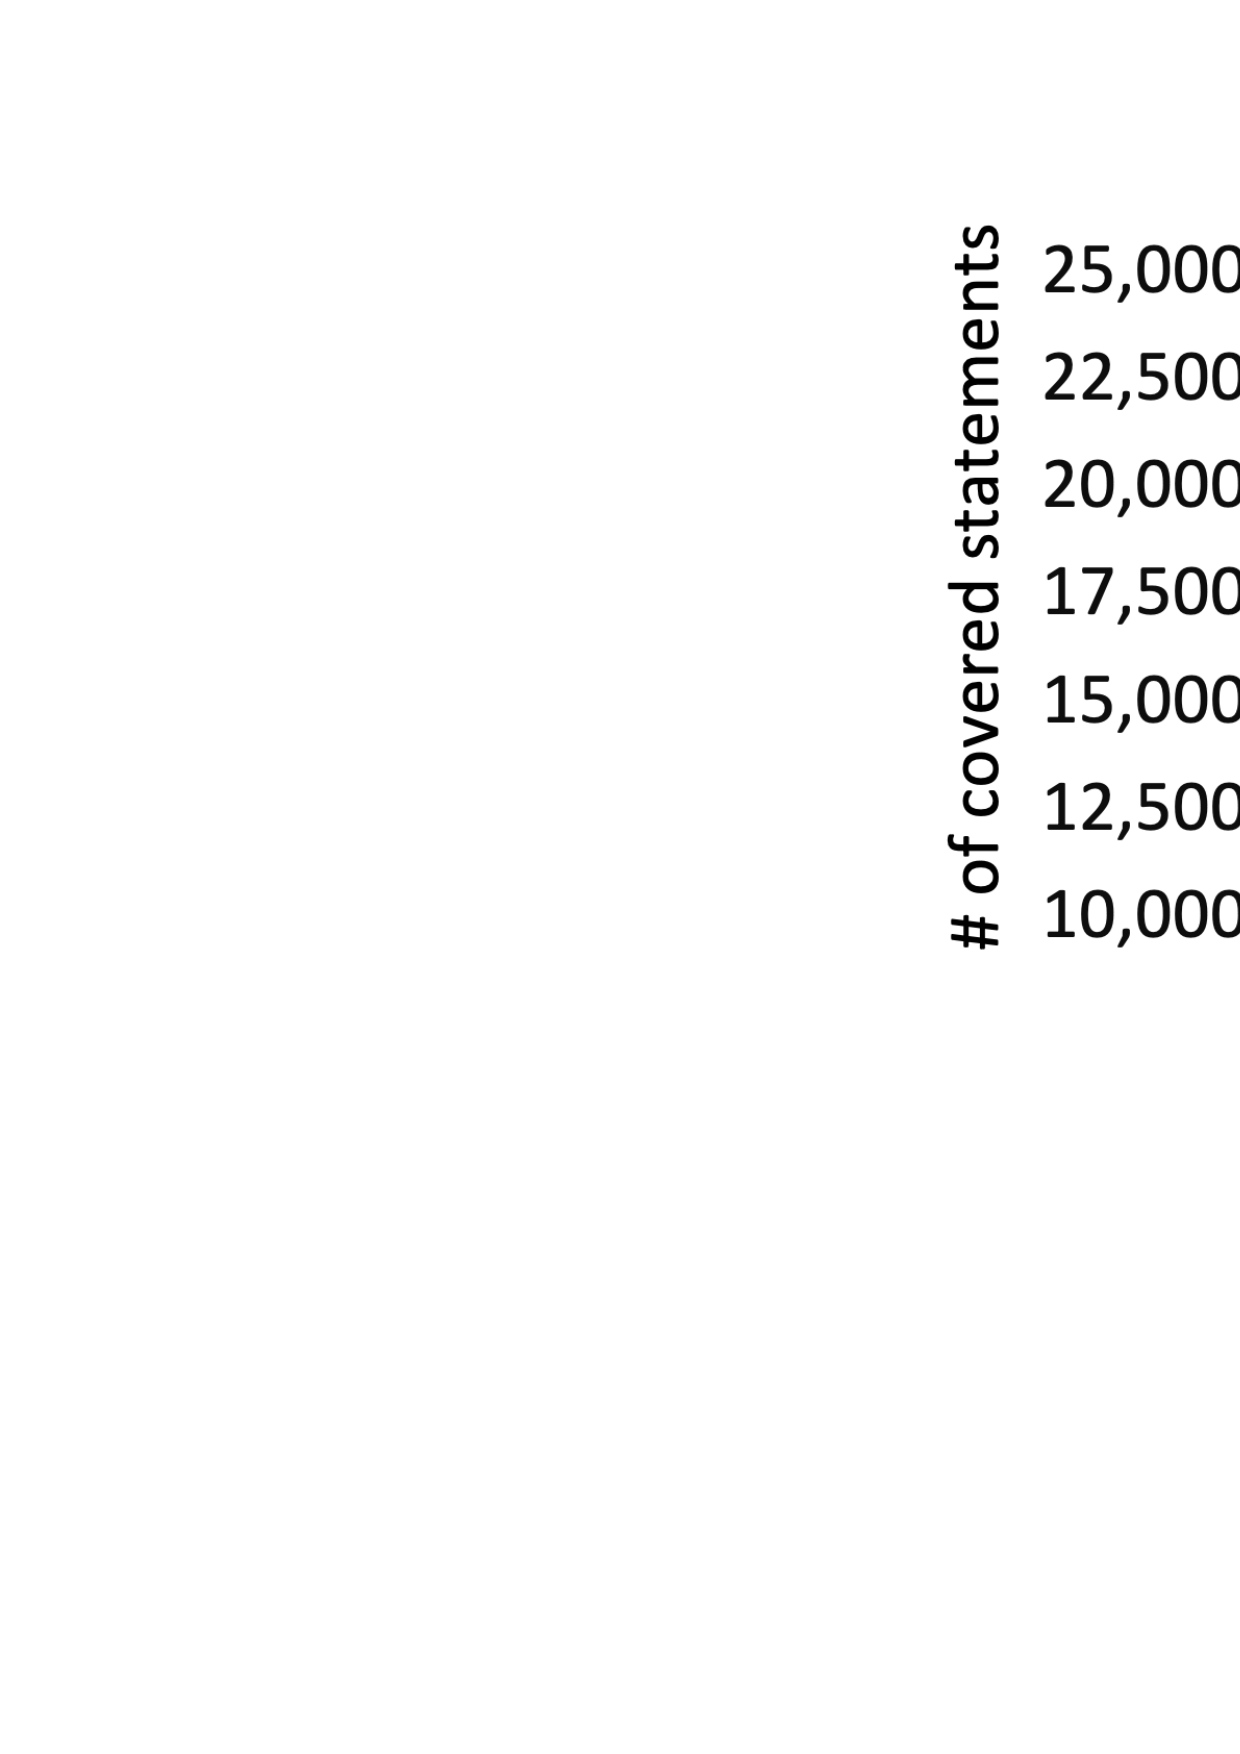
\includegraphics[width=\textwidth]{img/stmt-coverage.pdf}
    \caption{The statement coverage}
    \label{fig:stmt-coverage}
  \end{subfigure}
  \quad
  \begin{subfigure}[t]{0.48\textwidth}
    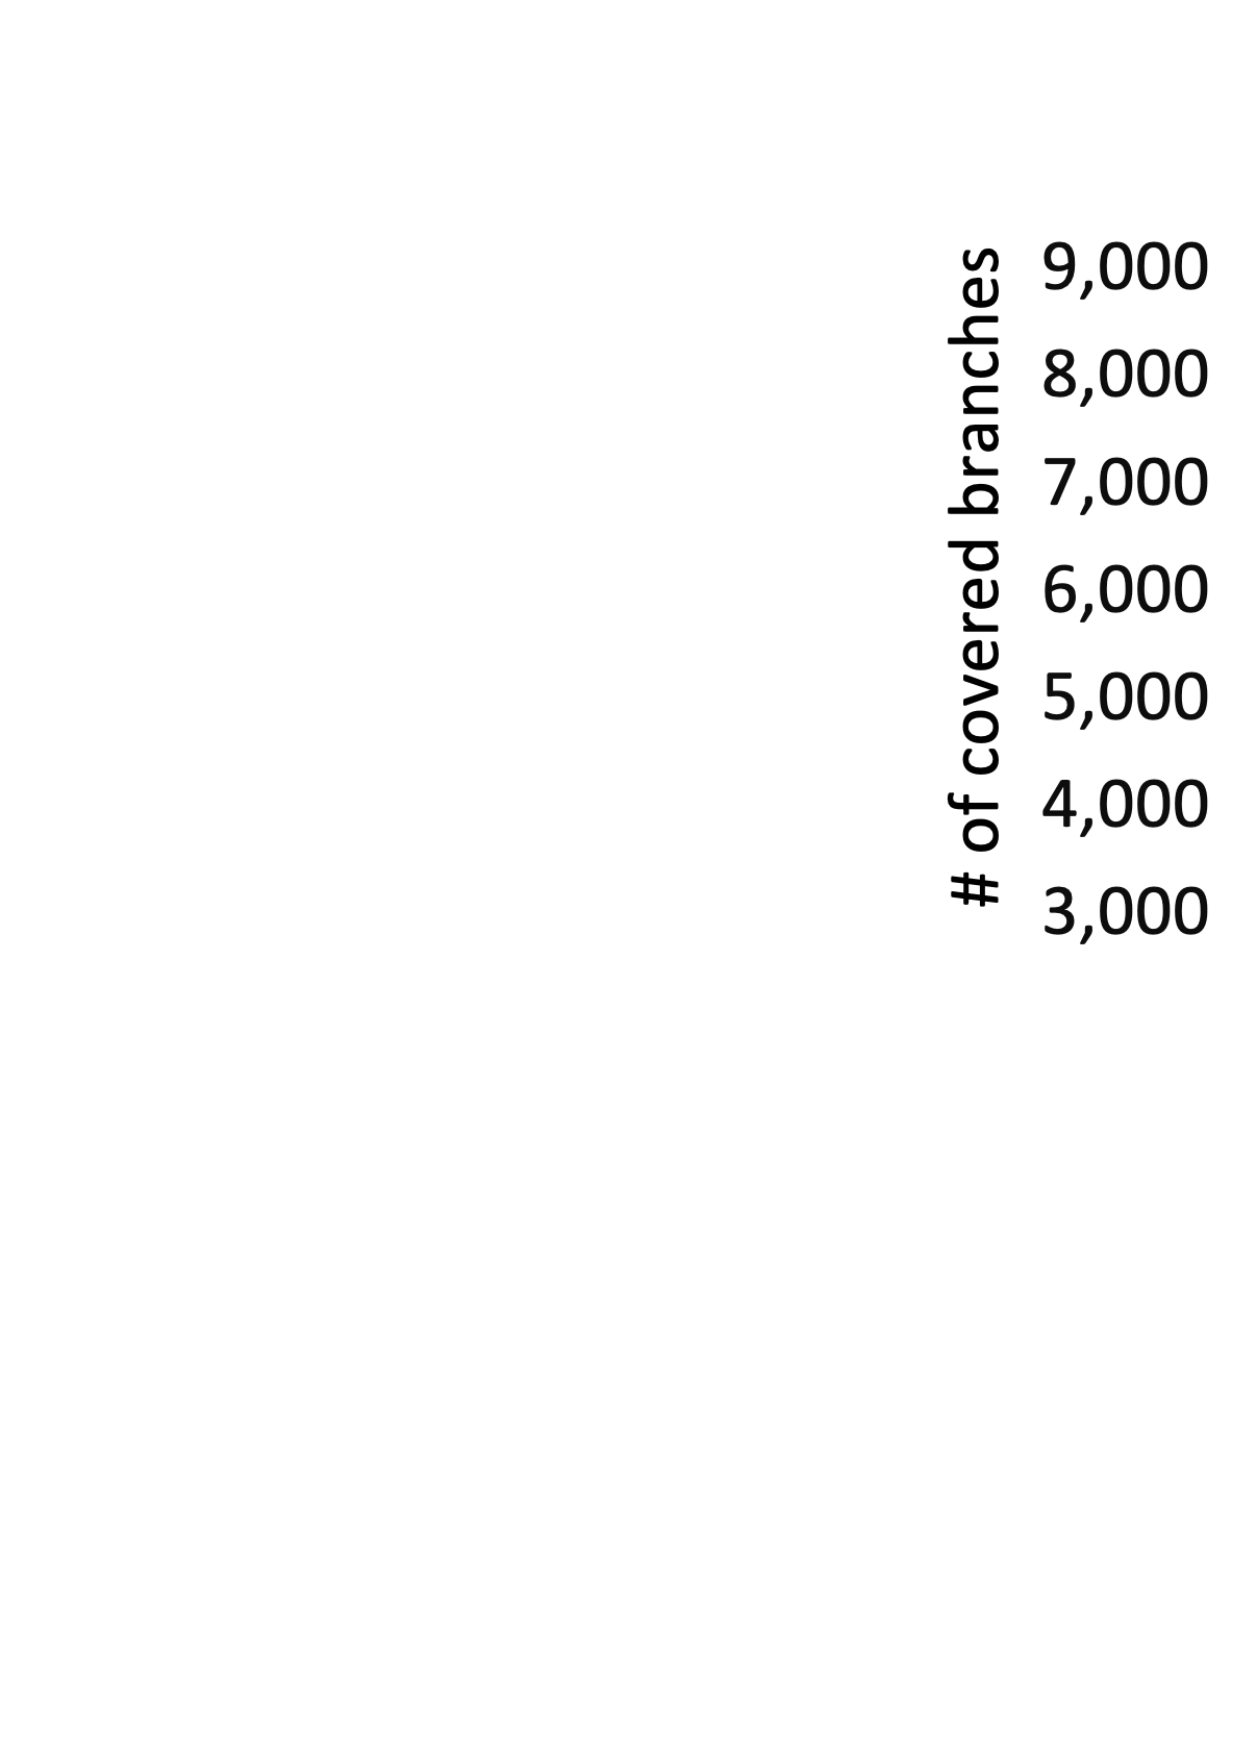
\includegraphics[width=\textwidth]{img/branch-coverage.pdf}
    \caption{The branch coverage}
    \label{fig:branch-coverage}
  \end{subfigure}
  \caption{The semantics coverage changes during the test generation phase}
  \label{fig:sem-coverage}
  \vspace*{-1em}
\end{figure*}

To evaluate $\tool$ that performs $N$+1-version differential testing of JavaScript
engines and its specification, we applied the tool to four JavaScript engines that
fully support modern JavaScript features and the latest specification,
ECMAScript 2020 (ES11, 2020).  Our experiments use the following four JavaScript
engines, all of which support ES11:
\begin{itemize}
  \item \textbf{GraalJS(v20.1.0)\footnote{https://github.com/graalvm/graaljs\#current-status}:} A JavaScript implementation built on
    GraalVM~\cite{graaljs}, which is a Java Virtual Machine (JVM) based on
    HotSpot/OpenJDK developed by Oracle
  \item \textbf{QuickJS(2020-04-12)\footnote{https://bellard.org/quickjs/}:} A small and embedded JavaScript engine developed by
    Fabrice Bellard and Charlie Gordon~\cite{qjs}
  \item \textbf{Moddable XS(v10.3.0)\footnote{https://blog.moddable.com/blog/xs10/}:} A JavaScript engine at the center of the Moddable
    SDK~\cite{xs}, which is a combination of development tools and runtime
    software to create applications for micro-controllers
  \item \textbf{V8(v8.5)\footnote{https://v8.dev/}:} An open-source high-performance engine
for JavaScript and WebAssembly developed by Google~\cite{v8}
\end{itemize}
To extract a mechanized specification from ECMAScript, we utilize the tool
$\jiset$, which is a JavaScript IR-based semantics extraction
toolchain, to automatically generate a JavaScript interpreter from ECMAScript.
To focus on the core semantics of JavaScript, we consider only the semantics of strict mode
JavaScript code that pass syntax checking including the EarlyError rules.  To
filter out JavaScript code that are not strict or fail syntax checking,
we utilize the syntax checker of the most reliable JavaScript engine, V8.
We performed our experiments on a machine equipped with 4.0GHz Intel(R) Core(TM)
i7-6700k and 32GB of RAM (Samsung DDR4 2133MHz 8GB*4).  We evaluated $\tool$
with the following four research questions:
\begin{itemize}
\item {\bf RQ1 (Coverage of Generated Tests)} Is the semantics
coverage of the tests generated by $\tool$ comparable to that of Test262,
the official conformance test suite for ECMAScript, which is manually written?
\item {\bf RQ2 (Accuracy of Bug Localization)} Does $\tool$ localize bug locations
accurately?
\item {\bf RQ3 (Bug Detection in JavaScript Engines)} How many
bugs of four JavaScript engines does $\tool$ detect?
\item {\bf RQ4 (Bug Detection in ECMAScript)} How many
bugs of ES11 does $\tool$ detect?
\end{itemize}


\subsection{Coverage of Generated Tests}

$\tool$ generates the seed programs via \mytextsf{Seed Synthesizer},
which synthesizes 1,112 JavaScript programs in about 10
seconds and covers 97.78\% (397/406) of reachable 
alternatives in the syntax productions of ES11.
Among them, we filtered out 600 programs not necessary to increase semantics
coverage and started the mutation iteration with 523 programs.
Figure~\ref{fig:sem-coverage} shows the change of
semantics coverage of the program pool during the iterative process in 100 hours.
The left and right graphs present the statement and branch coverages, respectively.
The top red line denotes the coverage of Test262,
dark gray X marks denote tests generated from ES11, and blue O marks denote
tests generated from ES11 after fixing bugs detected by $\tool$.
For the statement coverage, out of \inred{24,495} statements in ES11, Test262
covers \inred{22,440 (91.61\%)} statements.
The initial program pool covers \inred{12,768 (52.12\%)} statements
and the final program pool covers \inred{21,230 (86.67\%)} and
\inred{21,482 (87.70\%)} statements before and after fixing bugs, respectively.
For the branch coverage, out of \inred{9,596} branches in ES11, Test262
covers \inred{7,956 (82.91\%)} branches.
The initial program pool covers \inred{3,987 (41.55\%)} branches
and the final program pool covers \inred{7,480 (77.95\%)} and
\inred{7,514 (78.30\%)} branches before and after fixing bugs, respectively.

\begin{table}
  \caption{The number of successes and covered branches of mutation methods}
  \label{table:mutation-method}
  \vspace*{-1em}
  \small
  \[
    \begin{array}{l?r|r}
      \telembf{c?}{Mutation Method}      & \telembf{c|}{Success}  & \telembf{c}{Branch (Avg.)}\\\toprule\\[-1.4em]
      \text{Nearest Syntax Tree Mutation} & 459                   & 1,230 (2.68)\\\hline
      \text{Random Mutation}              & 337                   & 1,153 (3.42)\\\hline
      \text{Statement Insertion}          & 209                   & 650   (3.11)\\\hline
      \text{Object Substitution}          & 169                   & 491   (2.91)\\\hline
      \text{String Substitution}          & 3                     & 3     (1.00)\\\hline
      \hline
      \telembf{c?}{Total}                 & 1,177                 & 3,527 (3.00)\\
    \end{array}
  \]
  \vspace*{-3em}
\end{table}

Table~\ref{table:mutation-method} shows the number of successes and covered
branches for each mutation method during the test generation phase.  In total,
$\tool$ successfully synthesize 1,177 programs that cover 3,527
more branches than the initial program pool.  Among five mutation methods, the
nearest syntax tree mutation is the most contributed method (459
successes and 1,230 covered branches) and the least one is the string
substitution (3 successes and 3 covered branches).  On average,
3.00 branches are covered by one successful mutation.

Finally, $\tool$ generates 1,700 JavaScript programs and the average
length of generated programs is 62.31.  After injecting assertions by
\mytextsf{Assertion Injector}, generated programs become conformance tests and
their average length is 245.90.  Compared to Test262, the number of
generated tests are much smaller and their sizes also shorter than those of tests
in Test262.  Test262 provides 16,251 tests for the same range of
semantics and their average size is 1,276.10.


\subsection{Accuracy of Bug Localization}

\begin{figure}[t]
  \centering
  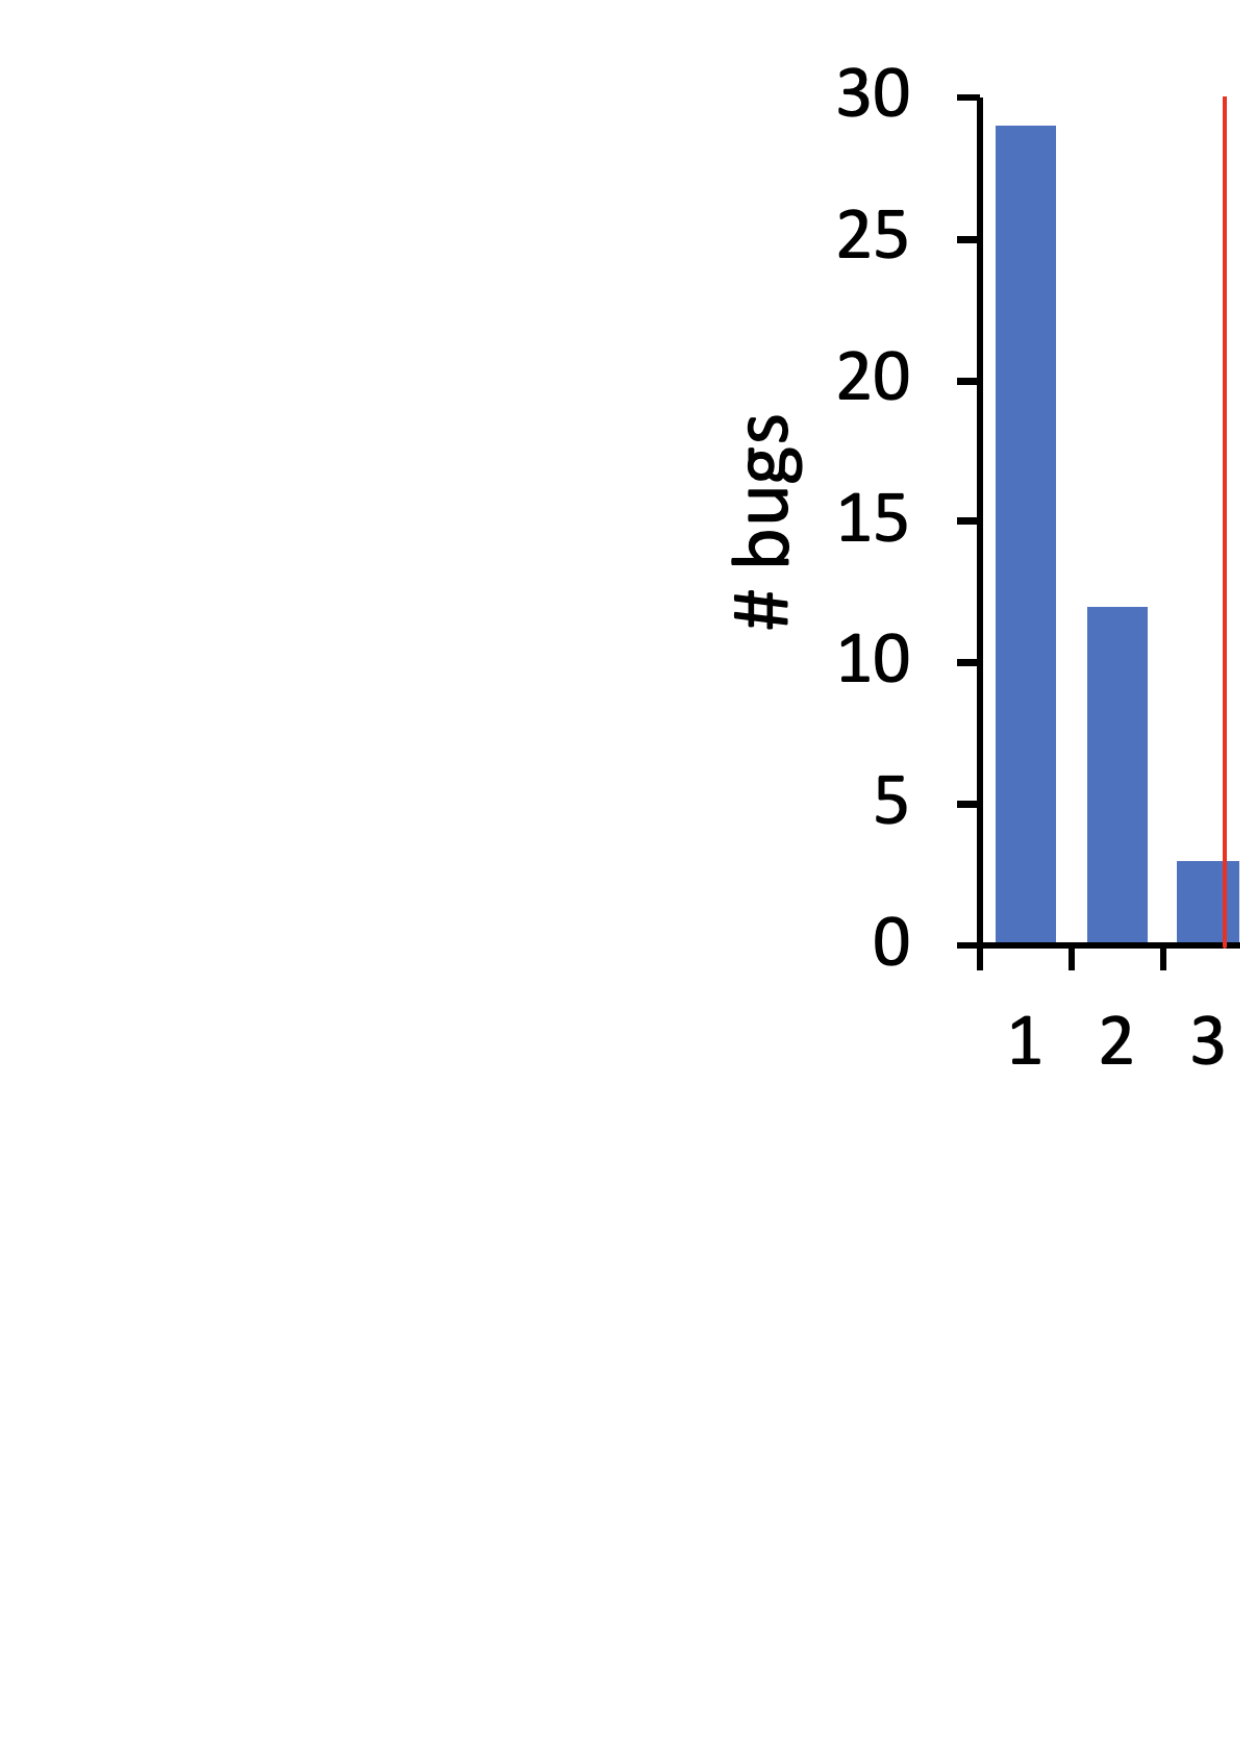
\includegraphics[width=0.48\textwidth]{img/localize.pdf}
  \caption{Ranks of algorithms that caused the bugs detected by $\tool$}
  \label{fig:localize}
  \vspace*{-1em}
\end{figure}

\setcounter{table}{2}
\begin{table*}[t]
  \centering
  \caption{Specification bugs in ECMAScript 2020 (ES11) detected by $\tool$}
  \label{table:spec-bug}
  \vspace*{-.5em}
  \small
  \begin{tabular}{@{}c@{~}?c|@{~}c@{~}|l|c|c|@{~}c@{~}|@{~}c@{~}|@{~}r@{}}
    \telembf{@{}c?}{\bf Name} &
    \telembf{c}{\bf Feature} &
    \telembf{@{}c@{~}}{\bf \#} &
    \telembf{c}{\bf Description} &
    \telembf{@{~}c@{~}}{\bf Assertion} &
    \telembf{@{~}c}{\bf Known} &
    \telembf{@{}c}{\bf Created} &
    \telembf{@{}c}{\bf Resolved} &
    \telembf{@{}c@{~}}{\bf Existed} \\\toprule\\[-1.4em]

    ES11-1 &
    \text{Function} &
    12 &
    \makecell[l]{Wrong order between property keys for functions} &
    \mytextsf{Key} &
    O &
    2019-02-07 &
    2020-04-11 &
    429 days \\\hline

    ES11-2 &
    \text{Function} &
    8 &
    \makecell[l]{Missing property \code{name} for anonymous functions} &
    \mytextsf{Key} &
    O &
    2015-06-01 &
    2020-04-11 &
    1,776 days \\\hline

    ES11-3 &
    \text{Loop} &
    1 &
    \makecell[l]{Returning iterator objects instead of iterator records\\
      in \textbf{ForIn/OfHeadEvaluation} for \code{for-in} loops} &
    \mytextsf{Exc} &
    O &
    2017-10-17 &
    2020-04-30 &
    926 days \\\hline

    ES11-4 &
    \text{Expression} &
    4 &
    \makecell[l]{Using the wrong variable \code{oldvalue} instead of\\
      \code{oldValue} in \textbf{Evaluation} of \textit{UpdateExpression}} &
    \mytextsf{Crash} &
    O &
    2019-09-27 &
    2020-04-23 &
    209 days \\\hline

    ES11-5 &
    \text{Expression} &
    1 &
    \makecell[l]{Unhandling abrupt completion\\
      in \textbf{Abstract Equality Comparison}} &
    \mytextsf{Exc} &
    O &
    2015-06-01 &
    2020-04-28 &
    1,793 days \\\hline

    ES11-6 &
    \text{Object} &
    1 &
    \makecell[l]{Unhandling abrupt completion in \textbf{Evaluation} of\\
      \textit{PropertyDefinition} for object literals} &
    \mytextsf{Exc} &
    X &
    2019-02-07 &
    \inred{X} &
    \inred{X} days
  \end{tabular}
  \vspace*{-0.5em}
\end{table*}

\setcounter{table}{1}
\begin{table}
  \caption{The number of engine bugs detected by $\tool$}
  \label{table:engine-bug}
  \vspace*{-1em}
  \small
  \[
    \begin{array}{l?r|r|r|r|r|r|r?r}
      \telembf{@{}c@{~}?}{Engines} &
      \telemsf{@{~}c@{~}|}{Exc} &
      \telemsf{@{~}c@{~}|}{Crash} &
      \telemsf{@{~}c@{~}|}{Var} &
      \telemsf{@{~}c@{~}|}{Obj} &
      \telemsf{@{~}c@{~}|}{Desc} &
      \telemsf{@{~}c@{~}|}{Key} &
      \telemsf{@{~}c@{~}?}{In} &
      \telembf{@{~}c@{}}{Total}\\\toprule\\[-1.4em]

      \text{GraalJS}      & 6   & 0 & 0 & 0 & 2 & 8   & 0 & 16\\\hline
      \text{QuickJS}      & 3   & 1 & 1 & 0 & 0 & 2   & 0 & 6\\\hline
      \text{Moddable XS}  & 12  & 0 & 0 & 0 & 3 & 5   & 0 & 20\\\hline
      \text{V8}           & 0   & 0 & 0 & 0 & 0 & 2   & 0 & 2\\\hline
      \hline
      \telembf{c?}{Total} & 21  & 0 & 1 & 0 & 5 & 17  & 0 & 44\\
    \end{array}
  \]
  \vspace*{-1.5em}
\end{table}

To detect more bugs through high diversity of programs,
we repeat the conformance test generation phase in ten times.
We executed the generated conformance tests on four JavaScript engines
to find bugs in the engines and the specification.
After inferring locations of the bugs in the engines or the specification
based on the majority of the execution results, we manually checked
whether the bugs are indeed in the engines or the specification. 
The following table shows that our method works well:

\begin{table}[H]
  \centering
  \vspace*{-1em}
  \small
  \[
    \begin{array}{l?r|r|r|r?r?r}
      \telembf{c?}{\# Failed Engines} &
      \telembf{c}{1} &
      \telembf{c}{2} &
      \telembf{c}{3} &
      \telembf{c?}{4} &
      \telembf{c?}{Total} &
      \telembf{c}{Average} \\\toprule\\[-1.4em]

      \text{Engine Bugs}        & 38  & 6   & 0   & 0   & 44  & 1.14\\\hline
      \text{Specification Bugs} & 0   & 0   & 10  & 17  & 27  & 3.63\\
    \end{array}
  \]
  \vspace*{-1em}
\end{table}

\noindent
For engine bugs, the average number of engine failures is 1.14
while the average number of failed engines for specification bugs is 3.63.
As we expected, when most engines fail for a test, the specification
may have a bug.

Based on the results of conformance tests on four JavaScript engines, we localized
the specification or engine bugs on the semantics of ES11.
Among 71 bugs, 7 bugs are related to syntax thus we localized only 64 semantics bugs.
Figure~\ref{fig:localize} shows the ranks of algorithms that caues the semantics bugs.
The average rank is 3.19, and 82.8\% of algorithms causing
bugs are ranked in less than 5, 93.8\% in less than 10, and 98.4\% in less than 15.
Note that the location of one bug is ranked in 21 because of the limitation of SBFL;
its accuracy becomes low with a small number of failed test cases.



\subsection{Bug Detection in JavaScript Engines}
From four JavaScript engines, $\tool$ detected 44 bugs:
16 from GraalJS, 6 from QuickJS,
20 from Moddable XS, and 2 from V8.
Table~\ref{table:engine-bug} presents how many bugs for each assertion are detected
for each engine.  We injected seven kinds of assertions: exceptions
(\mytextsf{Exc}), crashes (\mytextsf{Crash}), variable values (\mytextsf{Var}), object
values (\mytextsf{Obj}), object properties (\mytextsf{Desc}), property keys
(\mytextsf{Key}), and internal methods and slots (\mytextsf{In}).
The effectiveness of bug finding is different for different assertions.
The \mytextsf{Exc} and \mytextsf{Key} assertions detected
engine bugs the most; out of 44 bugs, the former detected 21 bugs
and the latter detected 17 bugs.
\mytextsf{Desc} and \mytextsf{Var} detected 5 and 1 bugs, respectively, but the
other assertions did not detect any engine bugs.

We detected 16 engine bugs in GraalJS and one of them caused an engine
crash.  When we apply the prefix increment operator for \code{undefined}
as \code{++undefined}, GraalJS throws \code{java.lang.IllegalStateException}.
Because it crashes the engine, we cannot catch the exception using the
\code{try} statement:
\begin{lstlisting}[style=myJSstyle]
    try { ++undefined; } catch(e) { }
\end{lstlisting}
The GraalJS team has been fixing the bugs we reported and
asked whether we plan to publish the conformance test suite,
because the tests generated by $\tool$ detected many semantics bugs that
were not detected by other conformance tests:
\emph{``Right now, we are running Test262 and the V8 and Nashorn
unit test suites in our CI for every change, it might make sense to
add your suite as well.''}

In QuickJS, $\tool$ detected 6 engine bugs, most of which are due to corner cases of
the function semantics.  For example, the following code should throw
a \code{ReferenceError} exception:
\begin{lstlisting}[style=myJSstyle]
    function f (... { x = x }) { return x; } f()
\end{lstlisting}
because the variable \code{x} is not yet initialized when it tries to
read the right-hand side of \code{x = x}.
However, since QuickJS assumes that the initial value of \code{x} is
\code{undefined}, the function call \code{f()} returns \code{undefined}.
The QuickJS team confirmed our bug reports and it has been fixing the bugs.

$\tool$ found the most bugs in Moddable XS; it detected 20 bugs for various
language features such as optional chains, \code{Number.prototype.toString},
iterators of \code{Map} and \code{Set}, and complex assignment patterns.
Among them, optional chains are newly introduced in ES11, which shows that
our approach is applicable to finding bugs in new language features.
We reported all the bugs found, and the Moddable XS team has been
fixing them.  They showed interests in using our test suite:
\emph{``As you know, it is difficult to verify changes because the language specification
is so big. Test262, as great a resource as it is, is not definitive.''}

The most reliable JavaScript engine is V8 because $\tool$ found only two bugs and
the bugs are due to specification bugs in ES11.  Because V8 strictly follows the
semantics of functions described in ES11, it also implemented wrong semantics
that led to ES11-1 and ES11-2 listed in Table~\ref{table:spec-bug}.
The V8 team confirmed the bugs and fixed them.

\subsection{Bug Detection in ECMAScript}
From the latest ECMAScript ES11, $\tool$ detected 27 specification bugs.
Table~\ref{table:spec-bug} summarizes the bugs categorized by their root causes.
Among them, five categories (ES11-1 to ES11-5) were already reported and fixed in the current
draft of the next ECMAScript but ES11-6 was never reported before.
We reported it to TC39; they confirmed it and they will
fix it in the next version, ECMAScript 2021 (ES12).

ES11-1 contains 12 bugs; it is due to a wrong order between property keys of all kinds of
function values such as \code{async} and generator functions, arrow functions, and classes.
For example, if we define a class declaration with a name \code{A}
(\code{class A \{\}}), three properties are defined in the function
stored in the variable \code{A}: \code{length} with a number value \code{0},
\code{prototype} with an object, and \code{name} with a string \code{"A"}.
The problem is the different order of their keys because of
the wrong order of their creation.
From ECMAScript 2015 (ES6), the order between property keys is no
more implementation-dependent but it is related to the creation order of properties.
While the order of property keys in the class \code{A} should be \code{[length, prototype, name]}
according to the semantics of ES11, the order is \code{[length, name, prototype]}
in three engines except V8.  We found that it was already reported as a specification bug;
we reported it to V8 and they fixed it.
This bug was created on February 7, 2019 and TC39 fixed it on April 11, 2020;
the bug lasted for 429 days.

ES11-2 contains 8 bugs that are due to the missing property
\code{name} of anonymous functions.  Until ES5.1, anonymous functions, such as an identity arrow
function \code{x => x}, had their own property \code{name} with an empty string \code{""}.
While ES6 removed the \code{name} property from anonymous functions,
three engines except V8 still create the \code{name} property in anonymous functions.
We also found that it was reported as a specification bug and reported it
to V8, and it will be fixed in V8.

The bug in ES11-3 comes from the misunderstanding of the term ``iterator
object'' and ``iterator record''.  The algorithm \textbf{ForIn/OfHeadEvaluation}
should return an iterator record, which is an implicit record containing only internal slots.
However, In ES11, it returns an iterator object, which is a
JavaScript object with some properties related to iteration.
It causes a \code{TypeError} exception when executing the code \code{for(var x in \{\});} according to
ES11 but all engines execute the code normally without any exceptions.
This bug was confirmed by TC39 on April 30, 2020.

ES11-4 contains four bugs caused by a typo for the variable in the
semantics of four different update expressions: \code{x++}, \code{x--},
\code{++x}, and \code{--x}.  In each \textbf{Evaluation} of four kinds of
\textit{UpdateExpression}, there exists a typo \code{oldvalue} in step 3
instead of \code{oldValue} declared in step 2.  $\tool$ could not execute
the code \code{x++} using the semantics of ES11 because of the typo.
For this case, we directly pass the code to \mytextsf{Bug Localizer} to test whether the
code is executable in real-world engines and to localize the bug.
Of course, four JavaScript engines executed the update expressions without any issues
and this bug was confirmed by TC39 on April 23, 2020.

Two bugs in ES11-5 and ES11-6 are caused by unhandling of abrupt completions in
abstract equality comparison and property definitions of object literals, respectively.
The bug in ES11-5 was confirmed by TC39 and was fixed on April 28, 2020.
The bug in ES11-6 was a genuine one, and we reported it and received a confirmation
from TC39 on \inred{X}; the bug lasted for \inred{X} days.
